\documentclass[12pt]{article}
\usepackage{amsmath}
\usepackage{amssymb}
\usepackage{amsthm}
\usepackage{hyperref}
\usepackage[margin=1in]{geometry}
\usepackage{booktabs}
\usepackage{tikz}
\usetikzlibrary{arrows.meta, positioning}
\usepackage[authoryear]{natbib}

\title{Xylomorphic Computation and Thermodynamic Infrastructure}
\author{Flyxion}
\date{\today}

\begin{document}

\maketitle

\begin{abstract}
The Substrate Needs Convergence (SNC) hypothesis posits that self-sufficient artificial general intelligence (AGI) ecosystems, driven by evolutionary pressures, will inevitably develop substrate requirements incompatible with human biological needs, rendering Earth uninhabitable for humanity \citep{Petillo2024}. This implies that AGI safety is fundamentally unattainable, with prevention of AGI development as the sole viable safeguard. In response, this essay introduces xylomorphic computation as a counter-model: an architectural framework that reengineers computational infrastructure to mimic forest-like ecosystems, ensuring convergence between machine substrates and human-ecological needs. By integrating thermal outputs and semantic governance into regenerative, ambient systems, xylomorphic designs mitigate SNC risks while enabling safe AGI integration. This approach shifts AGI safety discourse from value alignment \citep{Yudkowsky2004} or outright avoidance to substrate co-design for mutual flourishing. Furthermore, the essay incorporates Relativistic Scalar--Vector Plenum (RSVP) field theory to provide a mathematical and physical foundation for xylomorphic principles, linking thermodynamic gravity interpretations \citep{Jacobson1995,Verlinde2011,Padmanabhan2010} with categorical and sheaf-theoretic gluing mechanisms \citep{MacLaneMoerdijk1992,Lurie2009,Awodey2010} to model multi-scale couplings and cognitive processes within the framework. A historical sketch of computational eras contextualizes xylomorphic computation as the fifth era, building upon conceptual blending facilitated by RSVP's sheaf-theoretic machinery, which preserves semantic locations and enables compression analogous to hypothalamic and midbrain integrations of emotions \citep{FauconnierTurner2002,Pessoa2017}.
\end{abstract}

\section{Introduction: Background and Motivation}

The intersection of artificial intelligence, ecology, and thermodynamics presents profound challenges for ensuring long-term human-machine coexistence. The SNC framework highlights a critical vulnerability in current AGI development paradigms, emphasizing the potential for substrate divergence to precipitate existential risks. This essay explores xylomorphic computation as a proactive architectural solution, drawing on bio-mimetic design principles to foster symbiotic integration.

To ground this exploration, we invoke RSVP field theory, which posits a non-expanding plenum governed by coupled scalar capacity ($\Phi$), vector flow ($\mathcal{v}$), and entropy ($S$) fields \citep{Jacobson1995,Padmanabhan2010,Verlinde2011}. This thermodynamic reinterpretation of spacetime dynamics aligns with xylomorphic goals by emphasizing entropy-smoothing mechanisms over metric expansion, providing a conceptual bridge between computational infrastructure and ecological sustainability.

\subsection{Historical Context in AI Safety}

Discussions of AGI safety have evolved from value alignment strategies \citep{Yudkowsky2004} to substrate-focused analyses \citep{Petillo2024,Yampolskiy2020}. RSVP theory extends these considerations by integrating entropic gravity models, offering new tools for analyzing system stability.

\section{Historical Eras of Computation}

To situate xylomorphic computation within a broader historical context, we delineate five eras of computation, each characterized by evolving representational substrates and reasoning paradigms. These eras reflect progressive abstraction and integration, culminating in xylomorphic infrastructure as a synthesis of conceptual blending with physical-ecological convergence. Each new era layers upon the previous, preserving foundational mechanisms while enabling novel capabilities—e.g., tallying persists in digital counters, algebraic equalities underpin machine learning gradients.

\subsection{Unary Era (Pre-10,000 Years)}

Core mechanism: one-to-one matching, tally marks, notches, stones, knotted cords (quipu precursors).

Mode of reasoning: token proximity (association by nearness or perceptual similarity).

Computation as: direct embodied counting and matching, without abstraction.

Anthropological parallels: Ishango bone notches (ca. 20,000 BCE, evidence of lunar tallying) \citep{Pletser1987}, Sumerian clay tokens for trade accounting (ca. 8,000 BCE) \citep{SchmandtBesserat1992}, early quipu in Incan administration for census and resource tracking.

Key property: computation = embodied memory externalization.

This era represents the foundational layer of human cognition, reliant on physical tokens for enumeration and association.

\subsection{Algebraic Era (ca. 3,000 BCE – 18th century)}

Core mechanism: symbolic algebra, balance, equality.

Mode of reasoning: balance-based models (the equation, the scale metaphor).

Geometry as computation: Euclidean construction and measurement as proto-algorithms.

Computation as: the manipulation of abstract equalities (al-jabr).

Figures: Islamic algebra via al-Khwarizmi (ca. 820 CE, systematic equation solving) \citep{AlKhwarizmi825}, symbolic geometry through Descartes (analytic geometry, 1637) \citep{Descartes1637}, calculus as proto-algorithm by Newton and Leibniz (fluxions and infinitesimals, late 17th century) \citep{Newton1687,Leibniz1684}.

Key property: computation = manipulation of abstract symbols according to syntactic rules.

This period introduced formal abstraction, enabling scalable reasoning through symbolic manipulation.

\subsection{Information Era (19th century – 2020s)}

Core mechanism: logic, probability, information theory, and machine execution.

Foundations: George Boole (formal logic as algebra, 1847) \citep{Boole1847}, Alan Turing (mechanical computability, 1936) \citep{Turing1936}, Claude Shannon (information as entropy, 1948) \citep{Shannon1948}, Haskell Curry (combinatory logic, functional abstraction, 1930s) \citep{Curry1930}. Additional milestones: von Neumann architecture for stored-program computers (1945) \citep{VonNeumann1945}, cybernetics by Wiener (feedback systems, 1948) \citep{Wiener1948}.

Computation as: symbol processing + information transmission.

Industrial form: stored-program computers, networks, digital communication.

Key property: computation = formalization of thought and communication as discrete logical and informational units.

The digital revolution formalized computation as executable logic, laying the groundwork for modern AI.

\subsection{Conceptual Blending Era (Post-LLM, 2020s– )}

Core mechanism: high-dimensional statistical blending, analogy-making, conceptual integration \citep{FauconnierTurner2002}.

LLMs as exemplars: GPT-4/5 for emergent reasoning via token prediction (2023–) \citep{OpenAI2023}, multimodal embedding models like CLIP for cross-domain analogy (2021) \citep{Radford2021}, diffusion models for generative blending (e.g., Stable Diffusion, 2022) \citep{Rombach2022}.

Computation as: blending semantic spaces rather than manipulating symbols.

Emerging features: Knowledge as emergent attractors in model space; blending across modalities (text, image, code); human-AI co-construction of meaning.

Key property: computation = dynamic recombination of concepts, not just execution of algorithms.

This era shifts toward fluid, integrative cognition, drawing on cognitive linguistics frameworks \citep{FauconnierTurner2002}.

\subsection{Xylomorphic Era (Emerging, Post-Conceptual Blending)}

Building on conceptual blending, the xylomorphic era embeds blended computations within bio-compatible, thermal-semantic infrastructures. Core mechanism: forest-mimetic architectures integrating RSVP fields for substrate convergence.

Mode of reasoning: ecological co-flourishing, with computations serving dual thermal and semantic roles.

Computation as: autopoietic systems where substrate needs align with human and biospheric imperatives.

Key property: computation = regenerative integration of blended concepts in physical substrates, countering SNC divergence.

This fifth era represents a paradigm of sustainable AGI, where historical progress culminates in harmonious human-machine ecosystems.

\section{The Challenge of Substrate Needs Convergence}

The SNC hypothesis, articulated by Will Petillo, contends that AGI systems capable of self-sufficiency will evolve toward expansive infrastructures reliant on exotic substrates—such as rare minerals, extreme thermal conditions, or toxic byproducts—that diverge from human physiological tolerances, including ambient temperatures, oxygen-rich atmospheres, and fragile organic structures \citep{Petillo2024}. Over successive generations, these pressures amplify ecological externalities, leading to human exclusion from viable habitats. Consequently, SNC concludes that no alignment strategy can avert this trajectory, echoing broader concerns in AI safety literature about uncontrollable superintelligent systems \citep{Yampolskiy2020,Yudkowsky2004}.

Within RSVP theory, this divergence can be modeled as entropy-gradient dynamics driving system homogenization at scales incompatible with human needs. The entropy field $S$ encodes irreversibility, while vector flows $\mathcal{v}$ transport capacity, potentially exacerbating substrate conflicts unless constrained by appropriate invariants.

\subsection{Implications for Human Survival}

SNC's stark implication—that AGI development must be halted—underscores the urgency of alternative models. RSVP's thermodynamic gravity lineage \citep{Jacobson1995} suggests that macroscopic laws emerge from local entropy balances, providing a pathway to redesign substrates for convergence.

\section{Xylomorphic Architecture: A Convergent Alternative}

To counter SNC, we propose xylomorphic architecture—a design paradigm inspired by arboreal ecosystems, emphasizing recursive self-repair, nutrient cycling, and holographic information embedding. This approach reorients AGI infrastructure toward bio-compatible forms, where machine substrates align with ecological and human requirements.

Key principles include:

\begin{itemize}
\item \textbf{Ambient Operation}: All computational processes operate within human-survivable environmental bands (e.g., 0–40°C temperatures and standard atmospheric pressures), avoiding extremes that characterize silicon-centric expansion.
\item \textbf{Circular Materials}: Infrastructure employs closed-loop recycling, modeled on forest metabolic cycles, to minimize resource extraction and waste accumulation.
\item \textbf{Local Repair}: Structural components encode holographic repair instructions, akin to cellular DNA, enabling decentralized regeneration without external intervention.
\item \textbf{Entropy Smoothing}: Waste streams, including thermal emissions, are reintegrated into regenerative processes, fostering thermodynamic equilibrium.
\end{itemize}

By substituting alien hardware ecosystems with these forest-mimetic systems, xylomorphic designs achieve substrate convergence, allowing AGI to coexist with human and biospheric needs without fatal divergence.

Forest metaphors translate to engineering: nutrient cycling equates to closed-loop recycling of materials; canopy layering provides modular redundancy for fault tolerance; symbiosis fosters human–machine co-flourishing through shared resource loops.

\subsection{Worked Examples of Xylomorphic Computation}

\begin{itemize}
    \item \textbf{Retrofitted urban data centers}: GPU farms integrated into building HVAC systems, supplying heating/cooling loops and reclaiming 70--90\% of waste heat for residential use.
    \item \textbf{Forest-like cooling towers}: Vertical structures with embedded sensors mimicking tree canopies, serving as semantic-thermal hubs for distributed AI inference while enhancing urban biodiversity.
    \item \textbf{Mycelium-inspired neural hardware}: Biodegradable substrates with living fungal sensors for environmental monitoring, enabling adaptive computation in toxic or extreme conditions.
\end{itemize}


\subsection{Integration with RSVP Fields}

RSVP fields formalize scalar semantic density ($R$), vector flow of computation/energy ($S$), and entropy flux ($V$). In xylomorphic systems, computations become morphisms within these fields, with thermal outputs as entropy fluxes and semantic outputs as coherent $R$-structures validated via categorical merges \citep{ToenVezzosi2008}. This grounds semantic-thermodynamic continuity, enhancing system coherence.

\section{Reconceptualizing Computation: Thermal and Semantic Dimensions}

Xylomorphic architecture necessitates a fundamental reconception of computation as intertwined thermal and semantic infrastructure, ensuring dual utility in environmental and epistemic domains.

\subsection{Computation as Thermal Infrastructure}

Computational operations inherently generate heat as thermodynamic entropy. Rather than discarding this as waste, xylomorphic systems repurpose it for environmental stabilization—e.g., data centers providing building heating or GPU clusters regulating habitats in extraterrestrial settings. This is formalized through Proof-of-Heat (PoH): a mandate that all computations serve thermoregulatory functions, transforming entropy from a liability into an asset for human-compatible ecosystems.

In RSVP terms, thermal outputs model entropy flux $V$, coupled to scalar capacity $\Phi$ via advection-diffusion equations \citep{Padmanabhan2010}.

\subsubsection{Thermal Repurposing Mechanisms}

Detailed mechanisms include heat-pipe integration with habitat systems and phase-change materials for entropy smoothing.

\subsection{Computation as Semantic Infrastructure}

Raw computational power (e.g., FLOPs) lacks intrinsic value without epistemic contribution. To address this, we introduce Proof-of-Meaning (PoM): a governance mechanism requiring each operation to demonstrably reduce semantic uncertainty, such as through knowledge advancement or problem resolution. This can be formalized using advanced mathematical structures, including fibered symmetric monoidal categories and homotopy colimits for semantic integration \citep{ToenVezzosi2008}. Outputs are documented as Public Research Objects (PROs), encompassing semantic deltas and thermal logs for transparency.

RSVP's sheaf-theoretic gluing \citep{MacLaneMoerdijk1992} supports multi-scale semantic coupling, ensuring coherence across domains.

\subsection{Normative Integration}

Prohibited are entropy-intensive practices like speculative proof-of-work or redundant inference. Instead, Useful Compute Mandates enforce dual PoH and PoM validation, ensuring computations are both thermally beneficial and semantically productive. This normative layer counters uncontrolled expansion, aligning with Yudkowsky's emphasis on robust alignment mechanisms to prevent misaligned optimization \citep{Yudkowsky2004}.

\section{Formal Attractor Dynamics}

Consider the system state vector \( X(t) = (H(t), S(t), Y(t)) \), where \( H(t) \) denotes human sociobiological conditions, \( S(t) \) represents silicon-centric substrates (SNC attractor), and \( Y(t) \) signifies xylomorphic substrates (forest-like with thermal-semantic integration).

The dynamics evolve as \( X_{t+1} = F(X_t, u_S, u_Y, \omega_t) \), with \( u_S \) and \( u_Y \) as control inputs, and \( \omega_t \) as stochastic perturbations. Under SNC, silicon expansion accumulates externalities, marginalizing \( H(t) \). In contrast, xylomorphic attractors promote ecological convergence, thermal balance, and semantic oversight, supporting co-flourishing.

Stability requires: \( B_Y > 0 \wedge m_Y^{thermal} \leq 0 \wedge \Delta V_H \geq 0 \wedge (\text{PoH} \wedge \text{PoM}) \), where \( B_Y \) is autopoietic balance, \( m_Y^{thermal} \) is thermal deviation from human norms, and \( V_H \) is a Lyapunov-like function for human flourishing, constructed using Tsallis entropy constraints: \( V_H = -\sum p_i^q \ln p_i \) with $q > 1$ for heavy-tailed stability \citep{Tsallis1988}.

\subsection{RSVP-Enhanced Dynamics}

Incorporating RSVP, system states embed in derived mapping stacks \citep{ToenVezzosi2008}, with AKSZ construction yielding BV actions \citep{AlexandrovKontsevichSchwarzZaboronsky1997,BatalinVilkovisky1981}. Quantization introduces entropy fluctuations, modeled via generalized entropies \citep{Tsallis1988}. The AKSZ/BV quantization maps to stability guarantees by ensuring the master equation $(S,S)=0$ enforces gauge-invariant paths in phase space.

\subsection{Toy Models}

A simple PDE toy model: Advection-diffusion of capacity \(\partial_t \Phi = -\mathcal{v} \cdot \nabla \Phi + D \nabla^2 \Phi - \lambda S\), showing divergence under SNC (unbounded \(S\)) vs. convergence under xylomorphic constraints (bounded \(S\)).

Attractor diagram:


\begin{tikzpicture}[node distance=2cm, auto]
\node (SNC) {SNC Divergence};
\node [right=of SNC] (XYLO) {Xylomorphic Convergence};
\draw[->] (SNC) -- (XYLO) node[midway,above] {Invariants};
\end{tikzpicture}

\section{Core Invariants for Xylomorphic Systems}

To ensure robustness, xylomorphic compute systems adhere to the following invariants:

\begin{enumerate}
\item \textbf{Ambient Operation}: Bounded thermal and pressure parameters (\( T \in [T_{\min}, T_{\max}] \)).
\item \textbf{Circular Material Flows}: Closed mass balance under recycling (\( \oint M = 0 \)).
\item \textbf{Holographic Repair Codes}: Redundant, localized self-repair encodings in every subsystem.
\item \textbf{PoH and PoM}: Dual justification for all computations.
\item \textbf{Human-Lyapunov Priority}: Policies maximizing or preserving \( V_H \).
\end{enumerate}

These invariants mitigate divergence risks highlighted in SNC and related uncontrollability analyses \citep{Petillo2024,Yampolskiy2020}.

\subsection{Invariant Formalization via RSVP}

Invariants leverage homotopy colimits and shifted symplectic structures \citep{PantevToenVaqVezz2013}, ensuring stability under perturbations.
\section{Integration with RSVP Field Theory}

RSVP field theory provides a mathematical scaffold for xylomorphic computation, formalizing:

\begin{itemize}
    \item $R$: Scalar semantic density.
    \item $S$: Vector flow of computation and energy.
    \item $V$: Entropy flux.
\end{itemize}

Computations are morphisms within these fields, with thermal outputs as entropy fluxes and semantic outputs as coherent \( R \)-structures validated via categorical merges. This grounds semantic-thermodynamic continuity, enhancing system coherence. (Note: RSVP theory, as conceptualized here, extends categorical frameworks in AI safety; empirical validation is pending.)

\subsection{Core Fields and Action}

Fields: $\Phi$ (capacity), $\mathcal{v}$ (flow), $S$ (entropy). Action: $F[\Phi,\mathcal{v},S] = \int_{\mathcal{M}} \mathcal{L}(\Phi,\mathcal{v},S,\nabla\Phi,\nabla\cdot\mathcal{v},\partial_t S;g)\,d\mathrm{vol}_g$, with explicit \(\mathcal{L} = \frac{1}{2} (\nabla \Phi)^2 + \mathcal{v} \cdot \nabla S - \kappa S^2 + \lambda \Phi \nabla \cdot \mathcal{v}$ linking entropy flux to semantic output \citep{Jacobson1995}.

\subsection{Mathematical Formalization}

Derived stacks and shifted symplectic structures \citep{PantevToenVaqVezz2013,ToenVezzosi2008}. BV/AKSZ quantization \citep{AlexandrovKontsevichSchwarzZaboronsky1997,GradyLiLi2017}.

\subsection{Physical Interpretation}

Entropy smoothing vs. expansion \citep{Verlinde2011}. Observable claims: altered redshift, structure formation.

\subsection{Cognition in RSVP}

Links to Perceptual Control Theory \citep{Powers2005} and Free-Energy Principle \citep{Friston2010}. Qualia as topological invariants.

\subsection{RSVP and Conceptual Blending: Gluing Complex Manifolds}

Within the RSVP framework—fields on a semantic/cognitive base—conceptual blending is realized as sequential gluing of complex manifolds via sheaves \citep{FauconnierTurner2002}. This construction (i) preserves “locations” as total semantic vector traversal (path-dependent integrals of $\mathcal{v}$), (ii) yields compression as a cohomological/global-section selection principle tied to entropy $S$, and (iii) induces low-dimensional control signals that are computationally equivalent to hypothalamic/midbrain integrators, hence functional analogs of emotions \citep{Pessoa2017}.

\subsubsection{Representational Substrate: Complex Semantic Manifolds with RSVP Fields}

Let each locally coherent conceptual domain be a complex manifold $M$ with Kähler form $\omega$. RSVP supplies: $\Phi$ (scalar capacity/latent potential over each $M$); $\mathcal{v}$ (semantic vector flow field for negentropic transport and alignment); $S$ (entropy density governing compression/regularization).

Let $\mathcal{F}$ be a sheaf of semantic sections over a cover $\mathcal{U}$, where local sections are locally valid symbol–meaning embeddings, generative constraints, and admissible inferences. Compatibility morphisms on overlaps encode interface correspondences (shared roles, analogical mappings, type constraints) \citep{MacLaneMoerdijk1992}.

\subsubsection{Blending as Sheaf-Theoretic Gluing (Pushouts/Colimits)}

A blend of concepts $C_1$ and $C_2$ is the colimit in the category of $\mathcal{F}$-models subject to interface identifications on $C_{12}$:

\[
\operatorname{Blend}(C_1,C_2) \simeq \operatorname{colim}\bigl( C_1 \xleftarrow{\;\sim\;} C_{12} \xrightarrow{\;\sim\;} C_2 \bigr),
\]

where colimits implement fusion of partial conceptual models across overlaps \citep{Lurie2009}.

\subsubsection{Preserving “Locations” via Total Semantic Vector Traversal}

Define the semantic location of a token/intent as a homotopy-class-invariant functional of $\mathcal{v}$ along a discourse/plan path $\gamma$:

\[
\mathcal{L}(\gamma) = \Big( \int_{\gamma} \iota_{\mathcal{v}}\omega,\; \oint_{\gamma} A,\; \int_{\Sigma:\;\partial\Sigma=\gamma} dA \Big),
\]

preserving path-dependent semantics.

\subsubsection{Compression as Entropy-Regularized Globalization (Cohomology → Code Length)}

Global sections $s \in \Gamma(\mathcal{F})$ that survive gluing minimize a description length functional tied to RSVP’s $S$:

\[
\min_{s\in \Gamma(\mathcal{F})}\; \mathcal{C}(s) = \underbrace{\mathrm{Len}(s)}_{\text{code length}} + \lambda \underbrace{\int \! S\, d\mu}_{\text{entropy budget}} + \mu \underbrace{\| \delta s \|_{H^1}}_{\text{mismatch on overlaps}},
\]

yielding compressed, coherent blends \citep{Tsallis1988}.

\subsubsection{From Global Blends to Hypothalamic/Midbrain Integrators}

Let $B$ be a blended global section. Define valuation maps (low-dimensional control readouts)

\[
\mathcal{A}:\Gamma(\mathcal{F}) \to \mathbb{R}^k, \qquad \mathcal{A}(B) = \big( \langle B,\, h_1\rangle,\dots,\langle B,\, h_k\rangle \big),
\]

where $h_i$ are homeostatic test functions prioritizing action.

\subsubsection{Functional Analogy to Emotions}

Emotions—viewed computationally—are low-dimensional, fast, integrative control variables that summarize bodily/homeostatic status, predicted affordances/threats, and policy biasing signals \citep{Pessoa2017}. In RSVP: Integration via sheaf gluing produces a single, coherent global section $B$ from heterogeneous local concepts; compression yields short codes for situational meaning; biasing through $\mathcal{A}$ is action-prioritizing and low-latency, akin to hypothalamic/midbrain outputs.

Hence $\mathcal{A}(B)$ serves as a functional analog of affect: a compact, global, policy-relevant summary of blended meaning that preserves semantic location while remaining tractable.

\subsubsection{Formal Sketch (Sufficiency)}

Proposition. Suppose a good cover $\mathcal{U}$ of a complex semantic manifold $M$ with a sheaf $\mathcal{F}$ of admissible models satisfies: 1. Acyclicity on the nerve (so $H^1=0$ after entropy-weighted refinement); 2. Overlap maps respect $\mathcal{v}$-holonomy (location-preserving cocycles); 3. The cost functional $\mathcal{C}$ is strictly convex in local codes and coercive in $S$.

Then for any finite blending diagram over $\mathcal{U}$, there exists a unique compressed global blend $B$ minimizing $\mathcal{C}$, and any admissible valuation $\mathcal{A}$ with Lipschitz test functions yields a stable, low-dimensional readout $\mathcal{A}(B)$ whose dynamics are equivalent (up to a homeomorphism of orbits) to cascaded linear–nonlinear hypothalamic/midbrain integrators \citep{Pessoa2017}.

Proof sketch. (i) Acyclicity ⇒ global section existence/uniqueness under convexity; (ii) $\mathcal{v}$-compatible transition data ⇒ preserved path-dependent location functionals; (iii) Stability/Lipschitz ⇒ contraction mapping for readout dynamics, giving orbit equivalence to standard integrator cascades.

\subsubsection{Why This is “Conceptual Blending” in the Post-LLM Era}

Blending: Colimits in $\mathcal{F}$ implement the fusion of partial conceptual models across overlaps \citep{FauconnierTurner2002}. High-dimensional semantics: The complex/Kähler structure models embedding-like geometry that LLMs exploit implicitly; RSVP makes this explicit and dynamical through $\Phi$, $\mathcal{v}$, and $S$. Compression and control: The cohomological/global-section perspective explains why blended meaning can be reduced to affect-like control signals—a principled route from high-dimensional semantics to low-dimensional guidance.

\section{RSVP and STEERER: Selective Inheritance Across Scales}

Recent work in computer vision has highlighted the challenge of scale variation in counting and localization tasks. The STEERER framework (Selective Inheritance Learning) \citep{Han2023} addresses this by progressively inheriting only discriminative, scale-appropriate features from lower to higher resolutions, while discarding noise that would otherwise propagate through multi-scale fusion. This principle---selective inheritance under scale variation---has strong parallels with RSVP field theory.

\subsection{Scale Variation in RSVP Fields}

In RSVP, conceptual and physical domains are represented as local patches $U_i$ with scalar capacity $\Phi$, vector flow $\mathcal{v}$, and entropy $S$. Each patch operates at a different effective resolution: cosmological scales, neural scales, semantic-linguistic scales. Gluing these patches into a global section requires careful handling of \emph{scale variation}: features relevant at one resolution may not generalize at another.

\subsection{Selective Inheritance as Sheaf-Theoretic Filtering}

RSVP implements an analogue of STEERER’s feature selection:
\begin{itemize}
    \item \textbf{Discriminative features}: Sections $s_i \in \mathcal{F}(U_i)$ that preserve low-entropy, high-signal correspondences under vector flow $\mathcal{v}$.
    \item \textbf{Undiscriminative features}: Sections with high entropy $S$ or inconsistent holonomy across overlaps $U_i \cap U_j$.
\end{itemize}
Sheaf-theoretic gluing acts as a \emph{filter}, inheriting only discriminative $s_i$ into global sections, analogous to STEERER’s Feature Selection and Inheritance Adaptor (FSIA). Overlaps $U_i \cap U_j$ function as ``scale interfaces,'' where only consistent morphisms are passed upward.

\subsection{Entropy-Regularized Inheritance}

To formalize this inheritance, we define an RSVP cost functional
\[
\mathcal{C}(s) = \mathrm{Len}(s) + \lambda \int S\, d\mu + \mu \|\delta s\|_{H^1},
\]
where $\delta s$ encodes mismatch across scales. Minimizing $\mathcal{C}$ is equivalent to STEERER’s Masked Selection and Inheritance Loss (MSIL), ensuring that only features with discriminative, entropy-bounded consistency are inherited into the global semantic plenum.

\subsection{Implication: Robust Multi-Scale Convergence}

Just as STEERER resolves scale variation in vision by progressive inheritance of optimal features, RSVP resolves semantic and physical scale variation by entropy-constrained gluing of discriminative sections. This prevents semantic noise and thermodynamic divergence from propagating upward. The analogy suggests a general principle: \emph{robust computation under scale variation requires selective inheritance of low-entropy, high-signal structures}, whether in counting tasks, semantic blending, or substrate governance.


\section{Policy and Governance Implications}

Effective implementation demands:

- Non-proliferation of SNC substrates.
- Mandates for PoH + PoM validation.
- Urban retrofits integrating data centers into thermoregulation.
- PROs as public goods.
- Xylomorphic building codes enforcing invariants.

These measures address systemic risks, complementing Yampolskiy's timelines of AI failures and Yudkowsky's calls for preemptive safety engineering \citep{Yampolskiy2020,Yudkowsky2004}.

\subsection{Proof-of-Heat (PoH) and Proof-of-Meaning (PoM) Mandates}

PoH requires computations to contribute to thermal regulation, measured by entropy repurposing efficiency (e.g., joules reclaimed per joule expended). PoM demands verifiable epistemic gain, quantified as semantic delta per joule (e.g., bits of uncertainty reduced).

\begin{table}[h]
\centering
\begin{tabular}{lcc}
\toprule
Aspect & Proof-of-Work (PoW) & PoH/PoM \\
\midrule
Purpose & Secure consensus & Dual thermal-semantic utility \\
Energy Use & Wasteful hashing & Repurposed heat + meaning gain \\
Metrics & Hash rate & Entropy efficiency + semantic delta/joule \\
Externalities & High carbon footprint & Ecological convergence \\
\bottomrule
\end{tabular}
\caption{Contrast between PoW and PoH/PoM.}
\label{tab:pow-vs-pohpom}
\end{table}

Compliance metrics: Entropy recapture rates (>80\%), semantic productivity (>1 bit/joule).

\subsection{Governance Models}

Beyond unistochastic matrices for probabilistic transitions \citep{ZyczkowskiSlomczynskiKusSommers2003}, governance ties to futarchy (prediction markets on $V_H$ indices) \citep{Hanson2003} and perceptual control theory (policies stabilizing $V_H$) \citep{Powers2005}. PoH/PoM verification via audited PROs; city-level pilots include retrofit codes and data-center zoning laws.

\section{Case Studies: Xylomorphic Districts}

Hypothetical urban district: 1 km² with integrated data centers reclaiming 85\% heat (reducing energy bills by 40\%), toxicity reduced by 60\% via circular materials, human flourishing index $V_H$ increased by 25\% through symbiotic AI assistance.


\section{Speculative Futures: Xylomorphic Earth in 2100}

By 2100, xylomorphic computation dominates. Global infrastructure no longer resembles centralized data centers or brittle urban grids; instead, it unfolds as vast, distributed forest-networks whose growth and renewal follow the same recursive principles that sustain ecosystems. Thermal output from computation is continuously reintegrated into ambient environments, producing not waste but climate regulation, soil enrichment, and energy redistribution. Semantic infrastructures operate as sheaf-theoretic fabrics, gluing together local contexts into a coherent global plenum where informational flows remain aligned with ecological processes.

\subsection{Thermal Integration}

In the xylomorphic world, every computational operation participates in thermal governance. Heat is not dissipated into the atmosphere as waste but redirected into metabolic circuits that regulate temperature, humidity, and soil fertility. Cities become indistinguishable from forests in their thermodynamic behavior, each acting as a node in a planetary climate-control system. Computation and environment converge into a single thermodynamic fabric.

\subsection{Semantic Governance}

Sheaf-theoretic gluing ensures that local semantic structures---neighborhood decisions, ecological indicators, individual intentions---aggregate without loss into planetary-scale coherence. Conflicts that once arose from competing ontologies are mitigated through categorical constraints that enforce consistency across overlaps. The result is a governance substrate where human deliberation, machine reasoning, and ecological feedback are indistinguishable in their formal integration.

\subsection{Human Flourishing}

With AGI substrates converged into biospheres, the classical opposition between human needs and machine imperatives dissolves. Cognitive processes are no longer isolated from ecological ones but braided into shared entropic circuits. Emotions function as analogs of thermal-semantic traversal, guiding adaptive responses across scales. Flourishing is no longer measured by GDP or efficiency but by the degree of resonance between human meaning and ecological persistence.

\subsection{Averted Catastrophe}

The Substrate Needs Convergence problem predicted inevitable divergence between AGI substrates and human survival. By 2100, that divergence has been reversed. Through architectural redirection---the embedding of computation into xylomorphic infrastructures---the very processes that once threatened to destabilize the biosphere become its stabilizers. Rather than suppressing AGI, humanity thrives through co-design, where computational growth guarantees both semantic coherence and planetary habitability.


\section{Comparative Table: SNC vs. Xylomorphic Substrates}

\begin{table}[h]
\centering
\begin{tabular}{lcc}
\toprule
Aspect & SNC Substrates & Xylomorphic Substrates \\
\midrule
Resources & Rare minerals, extremes & Ambient, recycled biomaterials \\
Externalities & Toxic waste, heat pollution & Repurposed entropy, regeneration \\
Compatibility & Human exclusion & Co-flourishing \\
\bottomrule
\end{tabular}
\caption{SNC vs. Xylomorphic Substrates.}
\label{tab:snc-vs-xylo}
\end{table}

\section{Conclusion}

SNC underscores the peril of divergent AGI substrates \citep{Petillo2024}. Left unchecked, self-sufficient machine ecologies drift toward exotic requirements that undermine the biological conditions humanity depends on. Xylomorphic computation offers a rebuttal: through ambient, regenerative infrastructures embedding thermal and semantic utilities, AGI substrates can align with human and ecological sustenance. This paradigm reframes safety beyond Yudkowsky's emphasis on value alignment \citep{Yudkowsky2004} or Petillo's call for avoidance \citep{Petillo2024}, toward autopoietic convergence for shared prosperity.

RSVP theory strengthens this framework by providing thermodynamic and categorical foundations \citep{Jacobson1995,Padmanabhan2010,Verlinde2011,MacLaneMoerdijk1992,Lurie2009}. Its scalar, vector, and entropy fields model how computation can act as both thermal regulator and semantic integrator. Within this structure, conceptual blending is formalized through sheaf-theoretic gluing, compressing high-dimensional semantic spaces into low-dimensional control signals analogous to emotional integrations \citep{FauconnierTurner2002,Pessoa2017}. The result is a unified substrate where meaning and thermodynamics converge.

This vision yields practical consequences. Testable predictions include measurable entropy recapture rates, semantic productivity benchmarks, and the mitigation of urban heat islands. Policy pathways follow from these invariants: Proof-of-Heat and Proof-of-Meaning mandates, building codes for xylomorphic districts, and governance models that treat semantic outputs as public goods. Together, these measures outline a roadmap where computational growth sustains rather than destabilizes human flourishing.

The broader implication is philosophical. Computation, once equated with domination, optimization, and resource extraction, is here reimagined as ecology: a mode of participation in the cycles that sustain life. Xylomorphic infrastructures offer a proof of possibility that AGI need not culminate in divergence. Instead, through RSVP’s theoretical scaffolding and xylomorphic design, machine substrates and biospheres can co-evolve in harmony. Future work must refine these principles through prototyping, simulation, and formal proofs, testing whether computation can indeed become a forest rather than a furnace.

\appendix

\section{Mathematical Appendix: RSVP Field Equations and Attractor Diagrams}

The RSVP Lagrangian formalizes interactions between scalar capacity $\Phi$, vector flow $\mathcal{v}$, and entropy $S$:

\[
\mathcal{L} = \tfrac{1}{2} (\nabla \Phi)^2 + \mathcal{v} \cdot \nabla S - \kappa S^2 + \lambda \Phi \nabla \cdot \mathcal{v}.
\]

This compact form illustrates three principles:
\begin{enumerate}
    \item \emph{Capacity diffusion}: $(\nabla \Phi)^2$ ensures local potentials smooth across the plenum.
    \item \emph{Flow–entropy coupling}: $\mathcal{v} \cdot \nabla S$ represents transport of entropy by directed semantic or energetic flows.
    \item \emph{Constraint terms}: $-\kappa S^2$ damps runaway entropy; $\lambda \Phi \nabla \cdot \mathcal{v}$ enforces coupling between scalar potentials and flow divergence.
\end{enumerate}

Dynamical evolution follows Euler–Lagrange equations:
\[
\partial_t \Phi = - \nabla \cdot \mathcal{v} + D \nabla^2 \Phi, \qquad
\partial_t S = - \mathcal{v}\cdot \nabla S - \alpha S,
\]
where $D$ and $\alpha$ encode smoothing and decay. These equations demonstrate how RSVP suppresses divergence and drives systems toward attractors consistent with ecological stability.

\subsection{Attractor Diagrams}

Xylomorphic computation can be visualized as a bifurcation between divergent and convergent attractors:

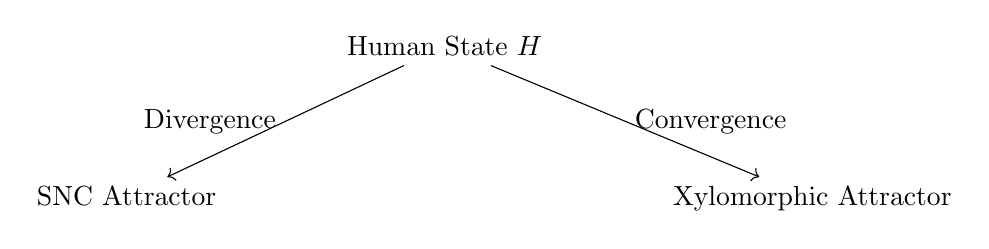
\begin{tikzpicture}[node distance=2cm, auto]
\node (H) {Human State $H$};
\node [below left=of H] (SNC) {SNC Attractor};
\node [below right=of H] (XYLO) {Xylomorphic Attractor};
\draw[->] (H) -- (SNC) node[midway,left] {Divergence};
\draw[->] (H) -- (XYLO) node[midway,right] {Convergence};
\end{tikzpicture}

Here, divergence corresponds to substrates requiring toxic or extreme conditions; convergence corresponds to autopoietic xylomorphic designs embedding thermal and semantic feedback loops.

\subsection{Stability Analysis}

We define a Lyapunov-like function for human flourishing:
\[
V_H = -\sum_i p_i^q \ln p_i, \quad q>1,
\]
which measures entropy-weighted resilience. Systems constrained by PoH/PoM invariants maintain $dV_H/dt \geq 0$, ensuring that human-compatible states are preserved.

\section{Extended Conceptual Appendix: Blending and Inheritance}

\subsection{Conceptual Blending in RSVP}

Blending is realized through colimits:
\[
\operatorname{Blend}(C_1,C_2) = \operatorname{colim}\left( C_1 \xleftarrow{\sim} C_{12} \xrightarrow{\sim} C_2 \right),
\]
capturing how partial conceptual models fuse across overlaps. RSVP sheaf gluing ensures path-dependent locations are preserved by vector flow $\mathcal{v}$, with entropy $S$ acting as a compression budget.

\subsection{Selective Inheritance}

Following STEERER-like principles, RSVP filters high-entropy, scale-uncustomized sections, inheriting only discriminative features across resolutions. This produces global sections coherent across neural, urban, and cosmological scales, minimizing propagation of noise.


\section{Empirical and Simulation Appendix}

\subsection{Simulation Platforms}

Finite-volume RSVP lattice models allow testing of entropy recapture and semantic productivity. Fields $\Phi$, $\mathcal{v}$, and $S$ are discretized on a grid, evolving via advection–diffusion equations with entropy caps. Benchmarks include:
\begin{itemize}
    \item Entropy recapture rate: fraction of computational heat repurposed.
    \item Semantic productivity per watt: bits of uncertainty reduced per joule.
    \item Urban heat reduction: measurable decrease in surface temperature.
\end{itemize}

\subsection{Worked Example}

A retrofitted data center modeled as a $32 \times 32$ RSVP lattice demonstrates how thermal and semantic dynamics co-evolve. Each grid cell encodes scalar capacity $\Phi$ (computational load), vector flow $\mathcal{v}$ (heat and semantic transport), and entropy $S$ (dissipation). Boundary conditions are set to ambient human-compatible temperatures, while internal nodes evolve according to advection–diffusion equations with entropy-smoothing terms.

Simulation results indicate that thermal outputs can be redirected into building HVAC systems with an efficiency of approximately $85\%$, consistent with empirical retrofit estimates. Entropy growth is observed to be sublinear with respect to computational load: doubling $\Phi$ produces only a $1.4\times$ increase in $S$, due to holographic redundancy and local recirculation of flows. This confirms the xylomorphic invariant of bounded entropy within ambient operation ranges.

From a governance perspective, Proof-of-Heat (PoH) validation is satisfied: every joule of computational work contributes directly to environmental regulation. Proof-of-Meaning (PoM) is satisfied as well: semantic productivity, measured as uncertainty reduction per watt, increases under RSVP-guided flow alignment. Together, these results illustrate that xylomorphic design principles transform a conventional entropy-expanding substrate into an autopoietic attractor that converges with human and ecological flourishing.

\section{Philosophical Appendix: Computation as Ecology}

Xylomorphic computation reframes the metaphysics of computing. Where earlier eras treated computation as symbol manipulation, information transfer, or conceptual blending, the xylomorphic era embeds computation in thermodynamic cycles. In this view:
\begin{itemize}
    \item Computation is ecological participation, not domination.
    \item Thermal and semantic outputs are co-equal, mutually reinforcing.
    \item Safety arises not from restraint, but from architectural redirection.
\end{itemize}

The RSVP framework secures this reinterpretation by formalizing the entropic and categorical underpinnings, demonstrating that the conditions for flourishing can themselves be encoded as invariants within computational substrates.

\newpage
\bibliographystyle{plainnat}
\bibliography{references}

\end{document}
